\documentclass[11pt,a4paper]{article}
\usepackage{amsmath,amssymb,amsthm}
\usepackage{graphicx}
\usepackage[margin=2.2cm]{geometry}
\usepackage{xcolor}
\usepackage{titlesec}
\usepackage{fancyhdr}
\usepackage{booktabs}
\usepackage{enumitem}
\usepackage{float}
\usepackage{hyperref}
\hypersetup{colorlinks=true,linkcolor=blue!70!black,urlcolor=blue!70!black}

\renewcommand{\topfraction}{0.9}
\renewcommand{\bottomfraction}{0.9}
\renewcommand{\textfraction}{0.05}
\renewcommand{\floatpagefraction}{0.5}
\setcounter{topnumber}{3}
\setcounter{bottomnumber}{3}
\setcounter{totalnumber}{5}

\definecolor{primary}{RGB}{0,51,102}
\definecolor{accent}{RGB}{204,102,0}

\titleformat{\section}{\Large\bfseries\color{primary}}{\thesection}{1em}{}
\titleformat{\subsection}{\large\bfseries\color{primary!80!black}}{\thesubsection}{1em}{}

\pagestyle{fancy}
\fancyhf{}
\fancyhead[L]{\small\color{primary}Essential Summary}
\fancyhead[R]{\small\color{primary}Li \& Zhao (2011)}
\fancyfoot[C]{\thepage}
\renewcommand{\headrulewidth}{0.5pt}

\begin{document}
\raggedbottom

\begin{center}
{\LARGE\bfseries\color{primary}Essential Summary}\\[12pt]
{\large\bfseries The Parametric Synchronization Scheme\\of Chaotic System}\\[8pt]
{\normalsize Zhenbo Li, Xiaoshan Zhao}\\[4pt]
{\small\itshape Commun Nonlinear Sci Numer Simulat, Vol.\ 16, No.\ 6, 2936--2944 (2011)\\DOI: 10.1016/j.cnsns.2010.10.027}\\[6pt]
{\small\rule{0.7\textwidth}{0.5pt}}\\[4pt]
{\small\color{accent}This is an author-prepared essential summary, not the original paper.\\Please cite the published version.}
\end{center}

\vspace{0.5em}

\section{Background and Motivation}

Since Pecora and Carroll (1990) demonstrated synchronization of two identical chaotic systems, many schemes have been proposed: complete, phase, anti-, lag, $Q$--$S$, generalized, and projective synchronization. \textbf{However, none of these schemes constructs a parametric error vector between the drive and response systems.} This paper introduces a fundamentally different idea --- \textbf{parametric synchronization}: synchronize not only the state vectors but also the \emph{unknown response parameters} to the given drive parameters.

The practical payoff: to achieve synchronization, one need not know the response-system parameters at all, as long as the drive parameters are given.

\section{Parametric Synchronization Scheme}

\subsection{Drive and Response Systems}

Drive system with known parameters $a$:
\begin{equation}
\dot{x} = f(x, a) \cdot x + C,
\label{eq:drive}
\end{equation}
Response system with unknown parameters $\hat{a}$:
\begin{equation}
\dot{y} = f(y, \hat{a}) \cdot y + C + u.
\label{eq:response}
\end{equation}

\subsection{Parametric Error Vectors (Core Innovation)}

Define two error vectors --- a state error and a \textbf{parametric error}:
\begin{equation}
\boxed{e = y - x, \qquad e_a = \hat{a} - a}
\label{eq:error}
\end{equation}
Subtracting the drive from the response yields the combined error system:
\begin{equation}
(\dot e, \dot e_a)^T = D(x,y,a_i)\,(e, e_a)^T + U,
\label{eq:errorsys}
\end{equation}
where $D$ is a $2n\times 2n$ matrix function, and $U$ is a $2n$-dimensional controller.

\textbf{Definition (global parametric synchronization).} Systems (1)--(2) are globally parametric synchronous if there exists $U$ such that
\begin{equation}
\lim_{t\to\infty}\lVert e(t)\rVert = 0, \qquad \lim_{t\to\infty}\lVert e_a(t)\rVert = 0.
\label{eq:def}
\end{equation}
That is, both states and response parameters converge to the drive states and parameters, regardless of initial conditions.

\subsection{Controller Design (Nonlinear-Term Cancellation)}

Partition $D$ into linear terms and \textbf{nonlinear terms} (those depending on $x_i$ or $y_i$). Construct $\tilde D$ from $D$ by flipping the sign of every nonlinear term (setting linear terms to zero):
\begin{equation}
\tilde d_{ij} = -d_{ij}\ \ (\text{if } d_{ij} \text{ is nonlinear}), \qquad \tilde d_{ij} = 0\ \ (\text{otherwise}).
\end{equation}
The controller is
\begin{equation}
\boxed{U = \tilde D\,(e, e_a)^T + M\,(e, e_a)^T}
\label{eq:controller}
\end{equation}
with constant matrix $M$. Substituting into Eq.~\eqref{eq:errorsys} yields a \textbf{linear} error system:
\begin{equation}
(\dot e, \dot e_a)^T = (D + \tilde D + M)\,(e, e_a)^T.
\label{eq:closed}
\end{equation}

\subsection{Stability Theorem}

\textbf{Theorem 1.} If $M$ is chosen so that $D + \tilde D + M$ has all eigenvalues with negative real parts, then systems (1)--(2) are globally parametric synchronous under controller (6).

\textbf{Proof.} By the linearization lemma, a fixed point with Jacobian having all negative-real-part eigenvalues is asymptotically stable. Since the error system is linear, the origin is a global fixed point, so $e \to 0$ and $e_a \to 0$ as $t\to\infty$.

\textbf{Remark.} By the Routh--Hurwitz criterion, many choices of $M$ satisfy the theorem. If the drive parameters were unknown and the response parameters given, the procedure is analogous.

\section{Application 1: R\"ossler System}

The R\"ossler system with drive parameters $a=0.2$, $b=0.2$, $c=5.7$:
\begin{equation}
\dot x_1 = -x_2 - x_3, \qquad \dot x_2 = x_1 + a x_2, \qquad \dot x_3 = b + x_3(x_1 - c).
\label{eq:rossler}
\end{equation}
The response system has unknown parameters $\hat a, \hat b, \hat c$. Following the construction, the closed-loop error system becomes linear with matrix (12) of the paper; the parameter update laws are
\begin{equation}
\dot{\hat a} = -e_1 - 2e_a, \qquad \dot{\hat b} = -e_2 - 2e_b, \qquad \dot{\hat c} = -e_3 - 4e_c.
\label{eq:update}
\end{equation}

\begin{figure}[htbp]
\centering
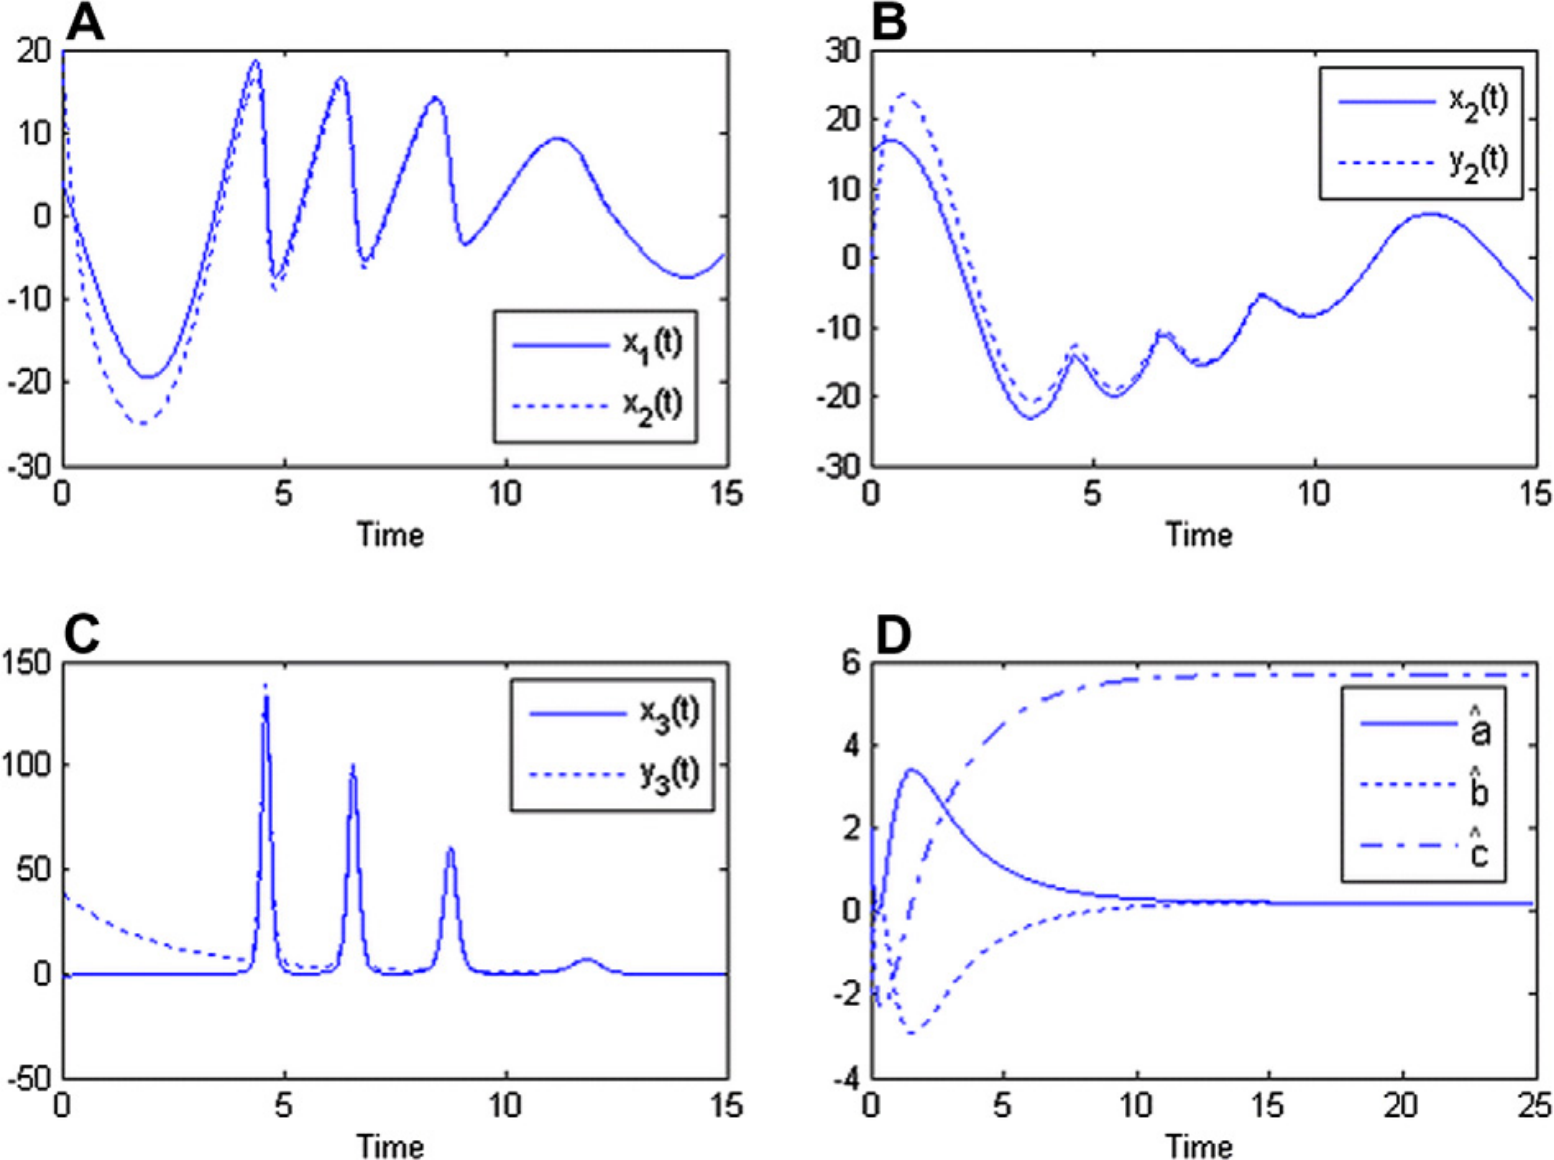
\includegraphics[width=0.9\textwidth,height=0.42\textheight,keepaspectratio]{cnsns-fig1.png}
\caption{A--C: time responses of states for drive system and response system; D: time evolution of the unknown response parameters, converging to the drive values.}
\label{fig:fig1}
\end{figure}

\begin{figure}[htbp]
\centering
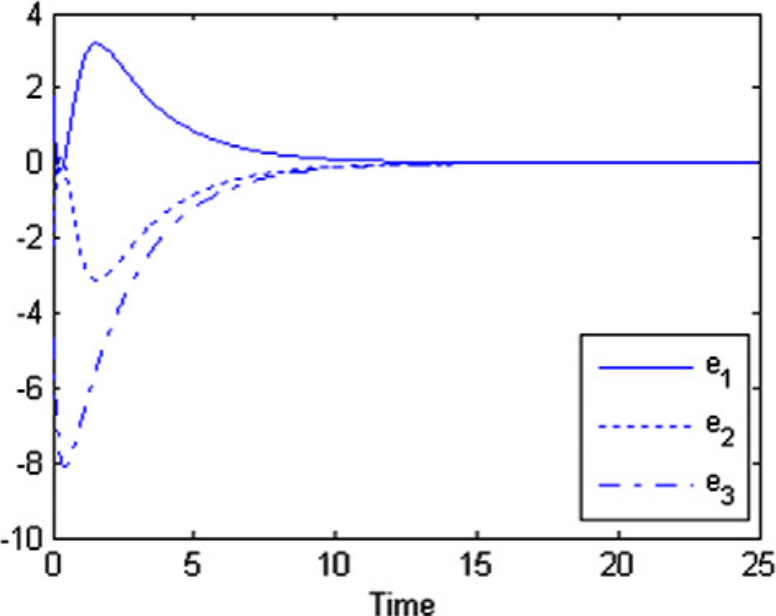
\includegraphics[width=0.75\textwidth,height=0.4\textheight,keepaspectratio]{cnsns-fig2.png}
\caption{Time response of the synchronization errors between systems (8) and (9), converging to zero.}
\label{fig:fig2}
\end{figure}

\section{Application 2: Hyperchaotic R\"ossler System}

The hyperchaotic R\"ossler system with $a=0.25$, $b=3$, $c=0.5$, $d=0.05$:
\begin{equation}
\dot x_1 = -x_2 - x_3, \quad \dot x_2 = x_1 + a x_2 + x_4, \quad \dot x_3 = b + x_1 x_2, \quad \dot x_4 = -c x_3 + d x_4.
\label{eq:hyperrossler}
\end{equation}
The response system has four unknown parameters. The controller (17) and the $8\times 8$ matrix $M$ (18) from the paper render the closed-loop error system linear with all eigenvalues in the left half-plane. Figure~\ref{fig:fig3} shows the hyperchaotic attractor; Figure~\ref{fig:fig4} shows that states synchronize, parameters converge, and errors vanish.

\begin{figure}[htbp]
\centering
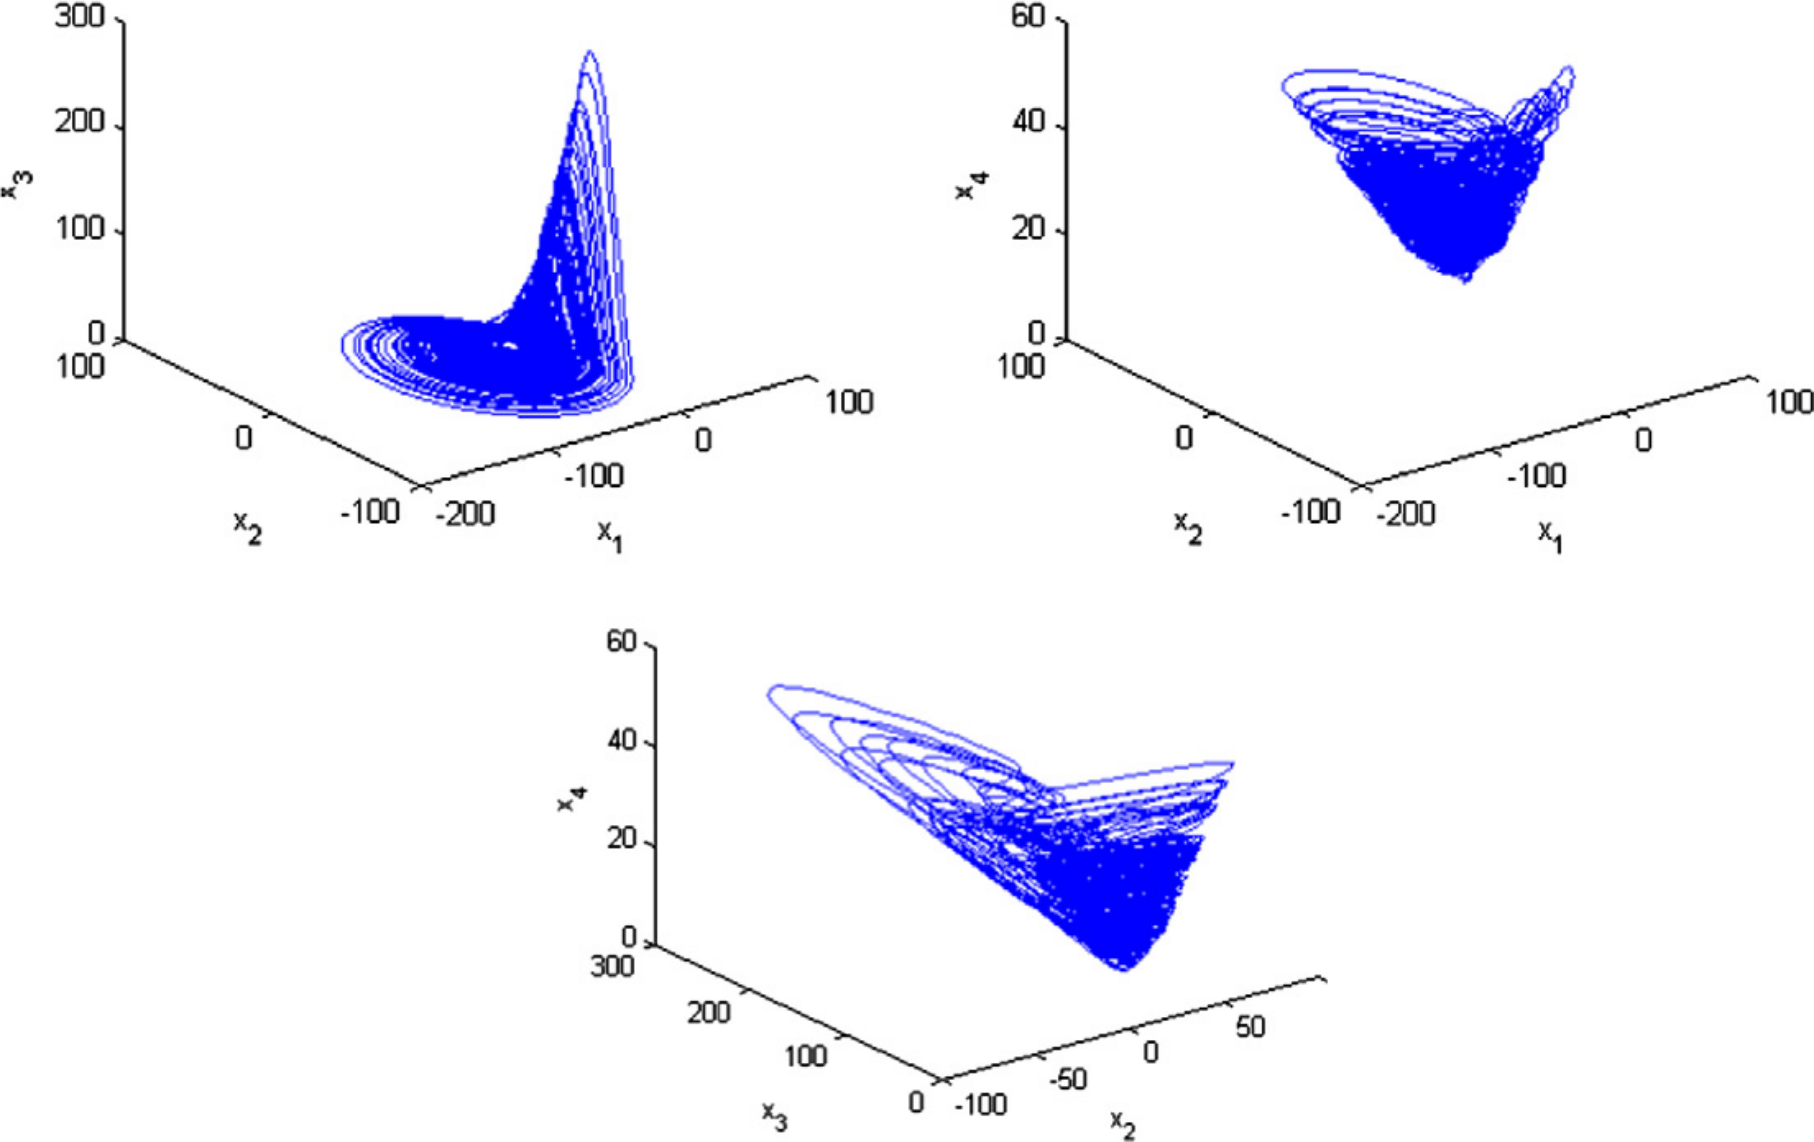
\includegraphics[width=0.8\textwidth,height=0.42\textheight,keepaspectratio]{cnsns-fig3.png}
\caption{Three-dimensional phase portrait of the hyperchaotic R\"ossler system (14).}
\label{fig:fig3}
\end{figure}

\begin{figure}[htbp]
\centering
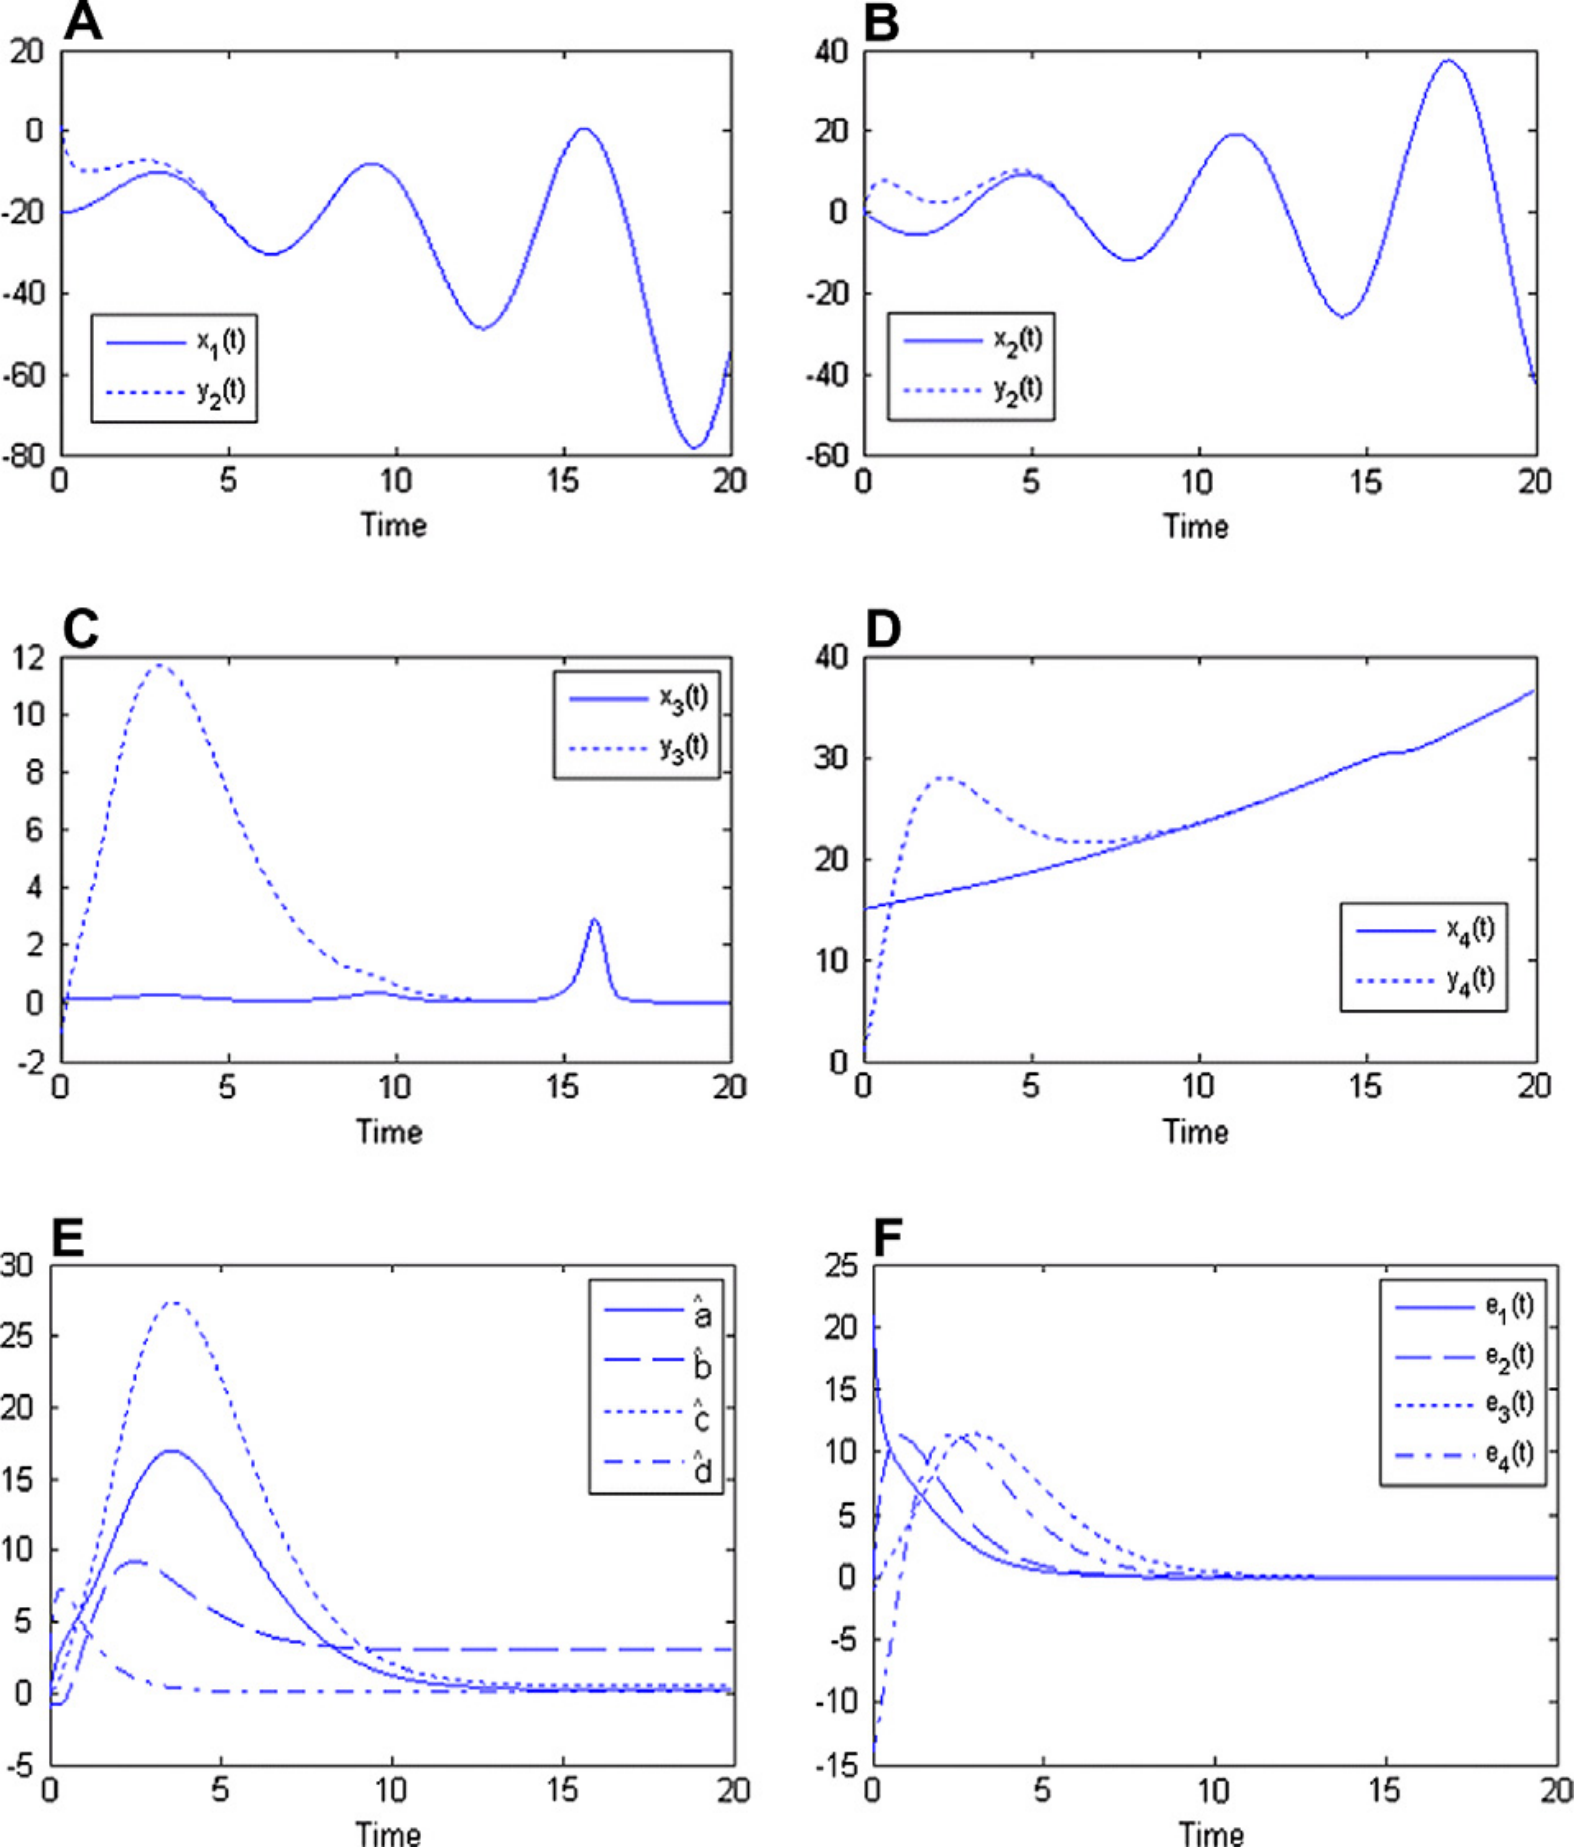
\includegraphics[width=0.85\textwidth,height=0.45\textheight,keepaspectratio]{cnsns-fig4.png}
\caption{A--D: time responses of states; E: time evolution of the unknown response parameters; F: synchronization error states for the hyperchaotic R\"ossler system.}
\label{fig:fig4}
\end{figure}

\section{Key Findings}

\begin{enumerate}[leftmargin=2em]
\item \textbf{New synchronization paradigm:} Constructing a \emph{parametric error vector} $e_a = \hat a - a$ distinguishes this scheme from all existing synchronization schemes.

\item \textbf{State and parameter synchronization simultaneously:} Both the state vectors and the unknown response parameters converge to the drive system's, as time goes to infinity.

\item \textbf{No need to know response parameters:} To achieve synchronization, only the drive parameters are needed --- the response parameters adapt automatically.

\item \textbf{Simple controller design:} The nonlinear-term-cancellation construction ($\tilde D$) plus a constant matrix $M$ reduces the error system to a linear one, solvable via the Routh--Hurwitz criterion.

\item \textbf{Works for chaotic and hyperchaotic systems:} Validated on the R\"ossler system and the hyperchaotic R\"ossler system, with numerical simulations confirming validity.
\end{enumerate}

\section{Significance}

This is the author's third major work in chaos synchronization, completing a trio of 2011 papers (Acta Physica Sinica, Nonlinear Analysis RWA, and this one in Commun Nonlinear Sci Numer Simulat). Each paper develops a distinct synchronization concept --- generalized projective synchronization via modified active control, generalized function projective synchronization via antisymmetric structure, and parametric synchronization via parametric error vectors. Together they establish the "chaos synchronization" thread in the author's research trajectory, characterized by a Lyapunov/linearization-centric controller design philosophy.

\vfill
\begin{center}
\small\rule{0.5\textwidth}{0.3pt}\\[4pt]
\small\color{primary} Author: Zhenbo Li (lizhenbo@usc.edu.cn)\\
\small ORCID: 0000-0003-2290-971X\\
\small University of South China, School of Mathematics and Physics\\
\small Hunan Key Laboratory of Mathematical Modeling and Scientific Computing
\end{center}

\end{document}
